
Neste seção, será descrito o possível impacto econômico da Pandemia de COVID-19, contextualizada na Seção~\ref{introducao:pandemia}, verificando mensalmente se o volume transacionado foi próximo ou não no volume esperado.

\section{Cenário geral}
\label{section:impacto:cenario-geral}

Nessa seção, descrevemos os dados da base totalizados mensalmente de forma agregada.

\begin{figure}[htb]
	\centering
    \caption{Valor total transacionado por mês no período analisado}
    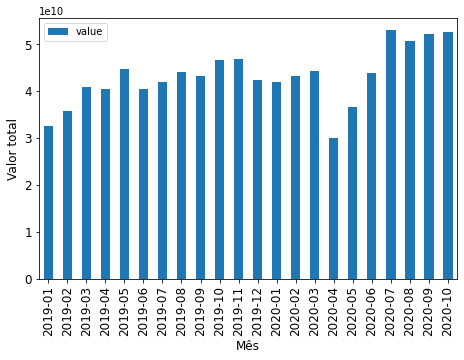
\includegraphics[scale=0.7]{images/base-de-dados-18.1-valor-mensal-total.png}
    \label{fig:pandemia:base-de-dados-18.1-valor-mensal-total}
    \fdadospesquisa
\end{figure}

\begin{figure}[htb]
	\centering
    \caption{Comparação do valor total transacionado por mês entre 2019 e 2020 (Parte 4)}
    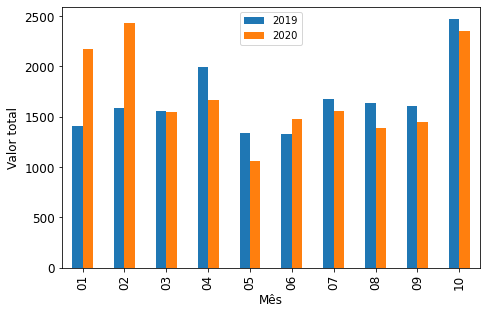
\includegraphics[scale=0.7]{images/base-de-dados-19.1-comparacao-valor-mensal-total.png}
    \label{fig:pandemia:base-de-dados-19.1-comparacao-valor-mensal-total}
    \fdadospesquisa
\end{figure}

A Figura~\ref{fig:pandemia:base-de-dados-18.1-valor-mensal-total} mostra o valor total transacionado em cada mês entre janeiro de 2019 e outubro de 2020, onde é visível um menor valor transacionado principalmente em abril e maio de 2020.

\begin{table}[htb]
\centering
\caption{Variação entre o valor transacionado para cada mês em 2020 em relação a 2019}
\label{tab:comparacao-valor-mensal-total}
\begin{tabular}{lr}
\toprule
Mês & Variação \\
\midrule
Janeiro &   25.49\% \\
Fevereiro & 14.58\% \\
Março &     12.71\% \\
Abril &    -12.24\% \\
Maio &     -11.24\% \\
Junho &      9.20\% \\
Julho &     11.64\% \\
Agosto &     7.52\% \\
Setembro &  17.02\% \\
Outubro &    3.33\% \\
\bottomrule
\end{tabular}
\fdadospesquisa
\end{table}

A Figura~\ref{fig:pandemia:base-de-dados-19.1-comparacao-valor-mensal-total} mostra uma comparação dos valores mensais transacionados em 2020 em relação aos valores mensais de 2019. Verifica-se então que os meses de abril e maio tiveram um valor total transacionado menor no ano de 2020, cuja variação por UF está descritos em detalhes na Tabela~\ref{tab:comparacao-valor-mensal-total}.

Como descrito na Seção~\ref{introducao:pandemia}, os meses de março e abril marcam exatamente o início do isolamento e das quarentenas no Brasil, e a aparentemente o impacto econômico nesses momentos foi mais importante.

Aplicando uma regressão linear a partir dos dados entre janeiro de 2019 e fevereiro de 2020 é possível obter uma da previsão de valor transacionado para os meses seguintes e então comparar com o valor obtido nos meses seguintes. Uma regressão linear não necessariamente é a melhor forma de prever o valor a ser transacionado para determinado mês, dados que os dados podem ter sazonalidades, porém se observarmos os dados da Figura~\ref{fig:pandemia:base-de-dados-18.1-valor-mensal-total}, podemos verificar uma tendência de crescimento linear mês a mês para os meses do ano de 2019. Isso não necessariamente ocorre porque houve um aumento real de transações das empresas envolvidas, mas porque a base de dados da empresa parceira tem crescido expressivamente mês a mês, com isso mesmo considerando o critério de recorrência, citado na seção~\ref{section:base-de-dados:dados-de-documentos-fiscais:preprocessamento}, a base de dados passa a receber mais dados de determinadas empresas, notoriamente aquelas que não são clientes da empresa parceira.

A Figura~\ref{fig:pandemia:base-de-dados-18.2-valor-total-vs-previsao} mostra os valores obtidos em relação aos valores previstos a partir da regressão linear aplicada sobre os dados, cuja variação é detalhada na na Tabela~\ref{tab:pandemia:valor-total-vs-previsao}.

\begin{figure}[htb]
	\centering
    \caption{Valor total transacionado por mês comparado com a previsão para o período analisado}
    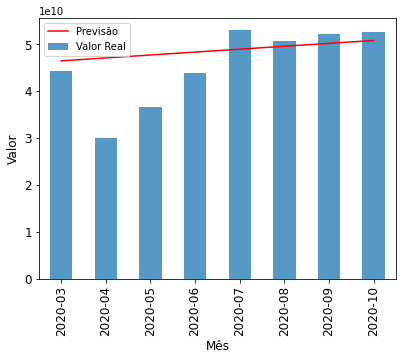
\includegraphics[scale=0.7]{images/base-de-dados-18.2-valor-total-vs-previsao.png}
    \label{fig:pandemia:base-de-dados-18.2-valor-total-vs-previsao}
    \fdadospesquisa
\end{figure}

\begin{table}[htb]
\centering
\caption{Variação entre o valor transacionado para cada mês em relação ao previsto após o início da pandemia}
\label{tab:pandemia:valor-total-vs-previsao}
\begin{tabular}{lr}
\toprule
Mês & Variação \\
\midrule
Março &     -4.46\% \\
Abril &    -36.22\% \\
Maio &     -23.11\% \\
Junho &     -9.15\% \\
Julho &      8.28\% \\
Agosto &     2.09\% \\
Setembro &   4.18\% \\
Outubro &    3.46\% \\ \hline
\textbf{Total} & -6.58\% \\
\bottomrule
\end{tabular}
\fdadospesquisa
\end{table}

A partir desses dados, é possível verificar que no período entre março e junho de 2020 o valor transacionado total foi menor que o previsto, verificando uma retomada posterior. Notoriamente, no mês de abril houve uma diferença de cerca de 36\% entre o valor previsto e o valor real. Dada essa leitura, vamos considerar posteriormente para efeitos de comparação que o segundo trimestre de 2020 foi o mais afetado economicamente pela pandemia, mesmo que no mês de março haja também impacto não o consideraremos pois as medidas de isolamento e distanciamento foram aplicadas apenas ao fim deste mês e o impacto não foi suficiente para alterar significativamente os totais do primeiro trimestre de 2020.

A partir de julho de 2020, o valor real transacionado foi maior que o valor previsto para esses meses. Isso pode indicar um menor impacto da pandemia para esses meses, e podemos observar na seção~\ref{introducao:pandemia} a partir da análise do índice de isolamento social que o isolamento social apesar de uma alta inicial em março e abril de 2020, começou a regredir a partir de julho de 2020, se mantendo estável após isso. Com isso, os níveis de consumo e produção possivelmente foram impactados positivamente com uma retomada, uma hipótese que ainda precisa ser mais lapidada uma vez que estamos analisando um período ainda limitado.

\section{Cenário regional}
\label{section:impacto:cenario-regional}

Nesta seção, descrevemos o impacto econômico da pandemia do ponto de vista regional. Usamos aqui a definição de região utilizada na seção~\ref{section:base-de-dados:analise-descritiva:abrangencia-territorial}. A Figura~\ref{fig:pandemia:base-de-dados-11.1-valor-total-por-regiao} mostra o valor total transacionado por região entre janeiro de 2019 e outubro de 2020 na base de dados utilizada neste trabalho.

\begin{figure}[htb]
	\centering
    \caption{Valor total transacionado por região no período analisado}
    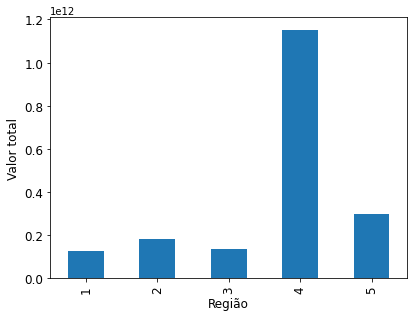
\includegraphics[scale=0.7]{images/base-de-dados-11.1-valor-total-por-regiao.png}
    \label{fig:pandemia:base-de-dados-11.1-valor-total-por-regiao}
    \fdadospesquisa
\end{figure}

A região 4 (sudeste) possui um valor transacionado muito maior em comparação às outras regiões. Segundo comparação feita na seção~\ref{section:base-de-dados:analise-descritiva:abrangencia-territorial}, não há uma preferência territorial clara para empresas da região sudeste possuindo um percentual de participação semelhante à de outras regiões. Esta região é conhecida por sua alta participação no cenário econômico brasileiro.

Na Figura~\ref{fig:pandemia:base-de-dados-21.1-valor-trimestral-por-regiao} é feita uma comparação trimestral entre o valor transacionado em cada um dos três primeiros trimestres de 2020 para cada região.

\begin{figure}[htb]
	\centering
    \caption{Valor trimestral transacionado por região no período analisado}
    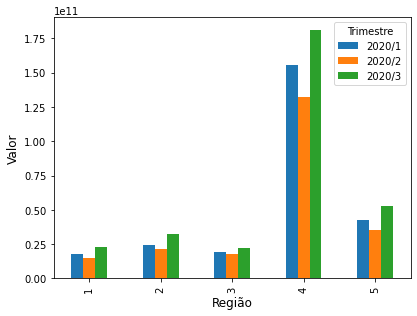
\includegraphics[scale=0.7]{images/base-de-dados-21.1-valor-trimestral-por-regiao.png}
    \label{fig:pandemia:base-de-dados-21.1-valor-trimestral-por-regiao}
    \fdadospesquisa
\end{figure}

Pode-se observar que todas as regiões tiveram um valor transacionado menor no segundo trimestre de 2020 em comparação aos outros dois trimestres analisados, o que indica um impacto econômico devido à crise causada pela pandemia, uma vez que os dados possuem uma tendência de crescimento no valor total transacionado, como argumentamos na seção~\ref{section:impacto:cenario-geral}.

A Tabela~\ref{tab:pandemia:variacao-por-regiao} descreve a diferença entre os valores previstos a partir de uma regressão linear aplicada sobre os dados de janeiro de 2019 a fevereiro de 2020 e àqueles obtidos para cada região entre março e outubro de 2020, da mesma forma como descrito na seção~\ref{section:impacto:cenario-geral}. Também é apresentada na mesma tabela a variação entre o valor total previto e obtido entre os meses de março a outubro de 2020.

\begin{table}[htb]
\centering
\caption{Diferença entre valores transacionados previstos e obtidos por região no período da pandemia}
\label{tab:pandemia:variacao-por-regiao}
\begin{subtable}[h]{\textwidth}
    \centering
    \begin{tabular}{c|r|r|r|r|r|r|r|r}
        \toprule
        \textbf{Região} & Março & Abril & Maio & Junho & Julho & Agosto & Setembro & Outubro \\
        \midrule
        \textbf{1} & -13.4\% & -48.8\% & -26.1\% &  -9.9\% &  8.9\% &  1.6\% &  0.7\% &  6.4\% \\
        \textbf{2} &  -9.2\% & -39.6\% & -22.3\% &  -5.3\% & 15.2\% & 10.1\% & 12.9\% & 18.9\% \\
        \textbf{3} &   8.2\% & -27.7\% & -10.7\% &   3.5\% &  9.6\% &  6.5\% &  8.4\% &  1.9\% \\
        \textbf{4} &  -3.0\% & -34.9\% & -23.8\% & -10.2\% &  3.0\% &  1.5\% &  3.4\% &  2.5\% \\
        \textbf{5} &  -8.5\% & -37.3\% & -24.9\% & -12.6\% & 22.5\% & -2.3\% &  1.6\% & -2.9\% \\
        \bottomrule
    \end{tabular}
    \caption{Diferença entre valor mensal previsto e obtido}
\end{subtable} ~ \\
\begin{subtable}[h]{0.45\textwidth}
    \centering
    \begin{tabular}{l|r}
        \toprule
        Região & Variação total \\
        \midrule
        \textbf{1} & -9.4\% \\
        \textbf{2} & -1.9\% \\
        \textbf{3} &  0.1\% \\
        \textbf{4} & -7.5\% \\
        \textbf{5} & -7.7\% \\
        \bottomrule
    \end{tabular}
    \caption{Diferença entre valor total previsto e obtido}
\end{subtable}
\fdadospesquisa
\end{table}

Verfificamos novamente que os meses mais impactados foram aqueles relativos ao segundo trimestre de 2020, de abril a junho. A diferença para o mês de abril chegou a ser de cerca de 48\% para a região 1 (norte), o que representa um impacto bastante significativo. É possível observar também cerca resiliência da região 3 (centro-oeste), sendo que essa região não apontou impacto no mês de março e foi capaz de se recuperar mais rapidamente já apresentando resultados positivos para o mês de junho. Com exceção da região 3, todas as regiões tiveram uma diferença entre o valor total previsto e o obtido para o período de março a outubro de 2020.

A Figura~\ref{fig:pandemia:base-de-dados-13-comparacao-valor-total-por-regiao} apresenta mês a mês o valor total transacionado em 2019 e 2020 para os meses de janeiro a outubro. Apesar da tendência de crescimento do valor transacionado mês a mês, o valor transacionado em abril e maio de 2020 foi menor que o valor transacionado em abril e maio de 2019 para todas as regiões.

\begin{figure}[htb] 
    \centering 
    \caption{Comparação do valor mensal transacionado por região entre 2019 e 2020}
    \label{fig:pandemia:base-de-dados-13-comparacao-valor-total-por-regiao} 
    \begin{subfigure}[b]{0.45\textwidth}
        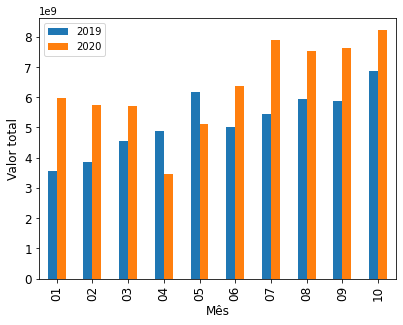
\includegraphics[scale=0.45]{images/base-de-dados-13.1-comparacao-valor-total-por-regiao.png}
        \caption{Região 1}
        \label{fig:pandemia:base-de-dados-13.1-comparacao-valor-total-por-regiao}
    \end{subfigure} ~ \quad
    \begin{subfigure}[b]{0.45\textwidth}
        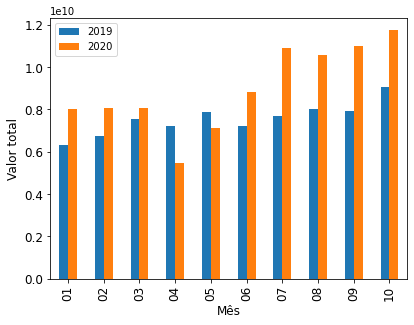
\includegraphics[scale=0.45]{images/base-de-dados-13.2-comparacao-valor-total-por-regiao.png}
        \caption{Região 2}
        \label{fig:pandemia:base-de-dados-13.2-comparacao-valor-total-por-regiao}
    \end{subfigure} ~ \\
    \begin{subfigure}[b]{0.45\textwidth}
        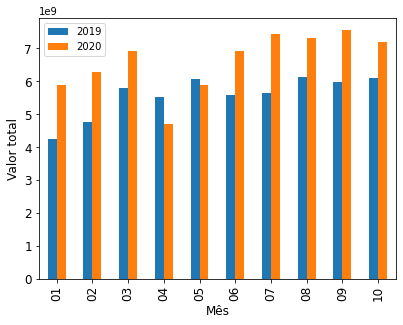
\includegraphics[scale=0.45]{images/base-de-dados-13.3-comparacao-valor-total-por-regiao.png}
        \caption{Região 3}
        \label{fig:pandemia:base-de-dados-13.3-comparacao-valor-total-por-regiao}
    \end{subfigure} ~ \quad
    \begin{subfigure}[b]{0.45\textwidth}
        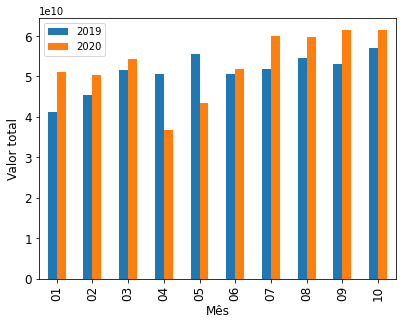
\includegraphics[scale=0.45]{images/base-de-dados-13.4-comparacao-valor-total-por-regiao.png}
        \caption{Região 4}
        \label{fig:pandemia:base-de-dados-13.4-comparacao-valor-total-por-regiao}
    \end{subfigure} ~ \\
    \begin{subfigure}[b]{0.45\textwidth} 
        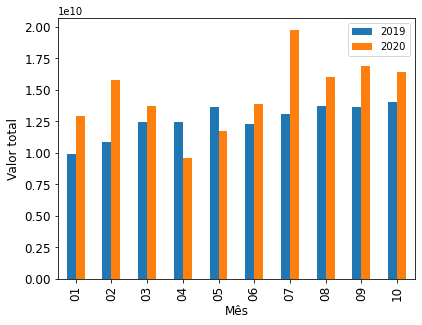
\includegraphics[scale=0.45]{images/base-de-dados-13.5-comparacao-valor-total-por-regiao.png}
        \caption{Região 5}
        \label{fig:pandemia:base-de-dados-13.5-comparacao-valor-total-por-regiao}
    \end{subfigure}
    \fdadospesquisa
\end{figure}

Na Figura~\ref{fig:pandemia:base-de-dados-14.1-valor-total-por-uf} vemos uma análise do valor total transacionado por UF no período de janeiro de 2019 e outubro de 2020. É possível observar um valor total transacionado consideravelmente maior no estado de São Paulo que, segundo descrição da seção~\ref{section:impacto:cenario-regional}, tem uma participação de 8\% do total das empresas deste estado, um percentual não muito diferente de outros estados citados. Outras UFs tem um valor total transacionado consideravelmente maior também, como Minas Gerais e Rio de Janeiro que reforçam a participação maior da região 4, e os estados da região 5 (sul): Paraná, Santa Catarina, e Rio Grande do Sul.

\begin{figure}[htb]
	\centering
    \caption{Valor total transacionado por UF no período analisado}
    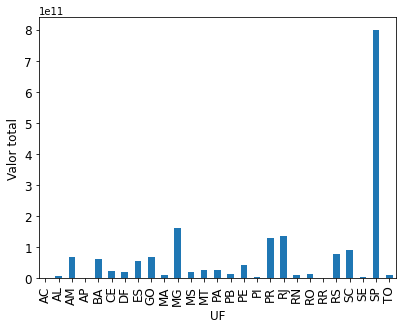
\includegraphics[scale=0.7]{images/base-de-dados-14.1-valor-total-por-uf.png}
    \label{fig:pandemia:base-de-dados-14.1-valor-total-por-uf}
    \fdadospesquisa
\end{figure}

A seguir, a Figura~\ref{fig:pandemia:base-de-dados-21.2-valor-trimestral-por-uf} apresenta graficamente uma comparação trimestral sobre o valor total transacionado em cada UF. Embora o valor total transacionado tenha grandes discrepâncias entre os estados, o que dificulta a identificação visual do impacto trimestral, é possível verificar que na maioria das UFs o valor total transacionado no segundo trimestre de 2020 é menor que no primeiro e no terceiro trimestre, o que indica um impacto maior devido à crise causada pela pandemia de COVID-19 nesse trimestre.

\begin{figure}[htb]
	\centering
    \caption{Valor trimestral transacionado por UF no período analisado}
    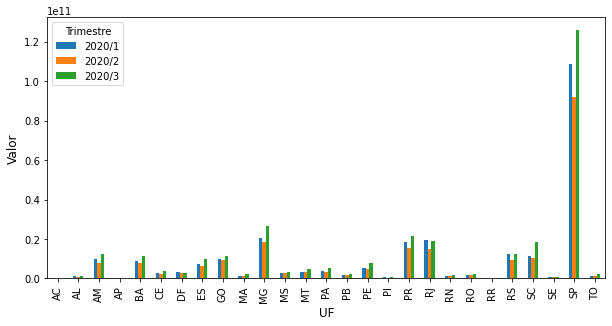
\includegraphics[scale=0.7]{images/base-de-dados-21.2-valor-trimestral-por-uf.png}
    \label{fig:pandemia:base-de-dados-21.2-valor-trimestral-por-uf}
    \fdadospesquisa
\end{figure}

Os dados são então detalhados na Tabela~\ref{tab:pandemia:variacao-mensal-por-uf}, onde é apresentada a diferença entre o valor mensal transacionado previsto para cada UF utilizando uma regressão linear sobre os dados entre janeiro de 2019 e fevereiro de 2020 e o valor real obtido para cada mês seguinte, de março a outubro de 2020.

\begin{table}[htb]
\centering
\caption{Diferença entre valores mensais transacionados previstos e obtidos por UF no período da pandemia}
\label{tab:pandemia:variacao-mensal-por-uf}
    \begin{tabular}{c|r|r|r|r|r|r|r|r}
        \toprule
        \textbf{UF} & Março & Abril & Maio & Junho & Julho & Agosto & Setembro & Outubro \\
        \midrule
        \textbf{AC} &  -7.3\% & -33.9\% &  -5.1\% &   9.2\% &   27.3\% &    20.5\% &    20.6\% &   15.4\% \\
        \textbf{AL} & -11.0\% & -33.6\% & -26.5\% & -12.3\% &    6.9\% &     3.9\% &    15.4\% &    9.0\% \\
        \textbf{AM} & -15.8\% & -62.5\% & -31.5\% & -14.3\% &    0.5\% &    -4.5\% &    -8.4\% &    4.1\% \\
        \textbf{AP} & -15.6\% & -29.1\% & -17.5\% &  -8.1\% &   17.4\% &    23.9\% &    22.1\% &   12.9\% \\
        \textbf{BA} &  -0.4\% & -36.0\% & -21.7\% &  -3.3\% &   11.0\% &     4.9\% &    12.7\% &   13.5\% \\
        \textbf{CE} & -15.6\% & -45.1\% & -26.3\% &  -7.7\% &   10.8\% &     7.6\% &     7.4\% &   19.1\% \\
        \textbf{DF} &  32.3\% & -18.6\% & -19.0\% &  16.4\% &    9.8\% &     2.8\% &    10.7\% &    6.6\% \\
        \textbf{ES} &  -6.5\% & -40.1\% & -24.2\% &  -5.8\% &    6.1\% &     5.6\% &    16.2\% &    6.4\% \\
        \textbf{GO} &  10.8\% & -29.5\% &  -7.9\% &   4.0\% &    9.5\% &     1.3\% &     7.3\% &    0.4\% \\
        \textbf{MA} & -20.9\% & -31.2\% & -24.8\% &   0.2\% &   22.3\% &    21.2\% &     6.8\% &   13.7\% \\
        \textbf{MG} &  -9.0\% & -35.1\% & -20.6\% &  -6.7\% &   12.2\% &     9.1\% &    12.0\% &   11.1\% \\
        \textbf{MS} &   3.4\% & -16.0\% &  -9.1\% &  -1.6\% &   12.8\% &     5.8\% &    -3.5\% &  -15.3\% \\
        \textbf{MT} & -13.3\% & -38.9\% & -13.4\% &  -3.2\% &    7.0\% &    24.5\% &    19.8\% &   17.0\% \\
        \textbf{PA} & -13.6\% & -33.3\% & -25.8\% &  -8.8\% &   18.5\% &     5.9\% &     9.7\% &    6.1\% \\
        \textbf{PB} &  -8.7\% & -38.5\% & -11.6\% &   1.7\% &   36.1\% &    15.8\% &    20.2\% &   30.7\% \\
        \textbf{PE} & -14.6\% & -43.4\% & -21.0\% &  -7.9\% &   17.5\% &    15.8\% &    11.8\% &   23.9\% \\
        \textbf{PI} & -10.6\% & -47.1\% & -24.5\% &  -7.0\% &   25.2\% &    13.4\% &    24.3\% &   15.1\% \\
        \textbf{PR} &  -2.2\% & -37.2\% & -22.8\% & -11.5\% &    1.5\% &    -0.7\% &     1.4\% &   -2.0\% \\
        \textbf{RJ} &  -6.7\% & -43.6\% & -25.6\% & -17.2\% &   -8.6\% &   -10.4\% &   -17.7\% &  -17.7\% \\
        \textbf{RN} & -14.9\% & -47.3\% & -39.7\% & -23.3\% &   10.6\% &     8.1\% &    24.7\% &   31.9\% \\
        \textbf{RO} &  -3.0\% & -25.2\% & -10.0\% &  -4.7\% &   17.1\% &     2.1\% &    -0.1\% &   -4.8\% \\
        \textbf{RR} &  82.5\% &  90.6\% & 189.3\% & 370.4\% & 1480.1\% & - & - & - \\
        \textbf{RS} & -18.4\% & -42.0\% & -33.7\% & -20.1\% &   -7.9\% &   -17.9\% &   -15.0\% &  -23.9\% \\
        \textbf{SC} &  -8.2\% & -32.5\% & -18.8\% &  -6.3\% &   89.5\% &    12.3\% &    20.3\% &   19.7\% \\
        \textbf{SE} &  -4.2\% & -38.7\% &   6.2\% &  23.9\% &   16.0\% &    13.6\% &     7.4\% &   26.6\% \\
        \textbf{SP} &  -0.9\% & -32.9\% & -24.1\% &  -9.9\% &    3.0\% &     1.9\% &     4.6\% &    4.1\% \\
        \textbf{TO} & -13.4\% & -32.1\% & -18.9\% &   2.4\% &   18.4\% &    13.9\% &    23.7\% &   19.7\% \\
        \bottomrule
    \end{tabular}
\nota{Os dados de Roraima foram insuficientes para uma previsão correta e registraram valores com bastante ruído, fazendo com que a previsão de valores utilizando a regressão linear indicasse valores bastante pessimistas para os meses da pandemia. Foram mantidos os valores de março a julho e removidos os valores posteriores devido ao ruído. Da mesma forma, consideramos que o estado de Roraima não foi impactado negativamente pela pandemia}
\fdadospesquisa
\end{table}

É possível observar que apenas o estado de Roraima não foi afetado pela crise segundo essa análise, mas como indicado na Tabela~\ref{tab:pandemia:variacao-mensal-por-uf} os dados desse estado não possuem um ruído considerável. Todos as outras UFs apresentaram pelo menos um mês cujo valor transacionado previsto e real indicam impacto negativo da crise. Os meses que concentram maior impacto novamente são os meses de março a junho, novamente indicando que o segundo de trimestre de 2020 foi o mais impactado pela pandemia.

Na Tabela~\ref{tab:pandemia:variacao-total-por-uf} apresentamos a diferença entre o valor total previsto e obtido para o período de março a outubro de 2020.

\begin{table}[htb]
\centering
\caption{Diferença entre valores totais transacionados previstos e obtidos por UF no período da pandemia}
\label{tab:pandemia:variacao-total-por-uf}
    \begin{tabular}{l|r}
        \toprule
        \textbf{UF} & Variação total \\
        \midrule
        \textbf{AC} &   6.2\% \\
        \textbf{AL} &  -5.5\% \\
        \textbf{AM} & -15.7\% \\
        \textbf{AP} &   1.3\% \\
        \textbf{BA} &  -1.8\% \\
        \textbf{CE} &  -5.7\% \\
        \textbf{DF} &   5.1\% \\
        \textbf{ES} &  -4.9\% \\
        \textbf{GO} &  -0.4\% \\
        \textbf{MA} &  -0.7\% \\
        \textbf{MG} &  -3.1\% \\
        \textbf{MS} &  -2.9\% \\
        \textbf{MT} &   0.4\% \\
        \textbf{PA} &  -4.6\% \\
        \textbf{PB} &   5.9\% \\
        \textbf{PE} &  -1.7\% \\
        \textbf{PI} &  -0.7\% \\
        \textbf{PR} &  -8.9\% \\
        \textbf{RJ} & -18.4\% \\
        \textbf{RN} &  -6.1\% \\
        \textbf{RO} &  -3.4\% \\
        \textbf{RR} & 484.7\% \\
        \textbf{RS} & -22.1\% \\
        \textbf{SC} &  10.0\% \\
        \textbf{SE} &   6.6\% \\
        \textbf{SP} &  -6.6\% \\
        \textbf{TO} &   2.5\% \\
        \bottomrule
    \end{tabular}
\fdadospesquisa
\end{table}

É possível verificar que dezoito UFs tiveram impacto no valor total transacionado em relação ao previsto, sendo os mais afetados o Rio Grande do Sul, o Rio de Janeiro, e o Amazonas. Nove UFs tiveram um valor previsto menor que o obtido, o que segundo esta análise significa que a retomada para estes estados pode ter compensado as perdas dos meses mais críticos.

Na Tabela~\ref{tab:pandemia:impacto-por-uf} é descrita a quantidade de UFs impactada mensalmente e totalmente no período analisado. Consideramos aqui que o impacto mensal significa que pelo menos um mês teve um valor transacionado obtido 25\% menor que o valor previsto, e impacto total indica que o valor total obtido foi menor que o previsto.

\begin{table}[htb]
\centering
\caption{Quantidade de UFs impactadas negativamente pela pandemia em relação às variações mensais ou totais}
\label{tab:pandemia:impacto-por-uf}
    \begin{tabular}{l|r|r}
        \toprule
        Impacto & Mensal & Total \\
        \midrule
        Sim & 24 & 18 \\
        Não &  3 &  9 \\
        \bottomrule
    \end{tabular}
\fdadospesquisa
\end{table}

\section{Cenário econômico}
\label{section:impacto:cenario-economico}

Nesta seção, serão apresentados os resultados da análise de impacto da pandemia de COVID-19 na economia do ponto de vista setorial. Para isso, vamos usar o CNAE para segmentar a economia, como descrito na seção~\ref{section:base-de-dados:analise-descritiva:abrangencia-economica}.

Na Figura~\ref{fig:pandemia:base-de-dados-15.1-valor-total-por-secao} é apresentado o volume transacionado por seção de CNAE considerando o total entre janeiro de 2019 e outubro de 2020.

\begin{figure}[htb]
	\centering
    \caption{Valor total transacionado por seção no período analisado}
    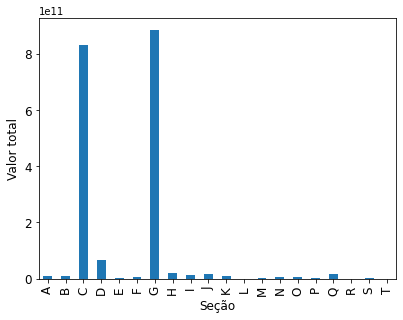
\includegraphics[scale=0.7]{images/base-de-dados-15.1-valor-total-por-secao.png}
    \label{fig:pandemia:base-de-dados-15.1-valor-total-por-secao}
    \fdadospesquisa
\end{figure}

A partir desses dados, podemos ver um volume muito maior transacionado nas seções C e G do CNAE, respectivamente as seções de "Indústria de Transformação" e "Comércio; Reparação de veículos automotores e motocicletas". Como pudemos ver na seção~\ref{section:base-de-dados:analise-descritiva:abrangencia-economica}, as seções C e G apresentam uma participação um pouco maior que as demais na base de dados, sendo que a seção G possui uma quantidade bastante grande de empresas também na base de referência em relação às demais, fato correspondido também aqui.

Na Figura~\ref{fig:pandemia:base-de-dados-22-valor-trimestral-por-secao} repetimos a análise trimestral agora por seção, ilustrando os valores transacionados nos três primeiros trimestres de 2020 para cada seção. Como as seções C e G possuem volumes muito maiores, é difícil visualizar o impacto para todas as seções, mas podemos verificar a mesma tendência encontrada até aqui: o segundo trimestre de 2020 apresentou um impacto negativo em relação ao primeiro e ao terceiro trimestres, com acentuada queda o volume transacionado total.

\begin{figure}[htb]
	\centering
    \caption{Valor trimestral transacionado por seção no período analisado}
    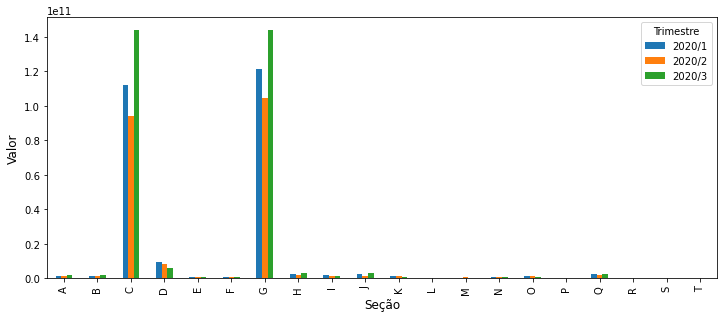
\includegraphics[scale=0.7]{images/base-de-dados-22-valor-trimestral-por-secao.png}
    \label{fig:pandemia:base-de-dados-22-valor-trimestral-por-secao}
    \fdadospesquisa
\end{figure}

Na Tabela~\ref{tab:pandemia:variacao-mensal-por-secao} é descrito em detalhes a diferença entre o valor previsto via regressão linear aplicada aos dados de valor mensal transacionado entre janeiro de 2019 a fevereiro de 2020 para os meses de março a outubro de 2020 e o valor obtido nesses meses.

\begin{table}[htb]
\centering
\caption{Diferença entre valores mensais transacionados previstos e obtidos por seção no período da pandemia}
\label{tab:pandemia:variacao-mensal-por-secao}
    \begin{tabular}{c|r|r|r|r|r|r|r|r}
        \toprule
        \textbf{Seção} & Março & Abril & Maio & Junho & Julho & Agosto & Setembro & Outubro \\
        \midrule
        \textbf{A} & -15.4\% & -24.4\% & -14.2\% & -10.8\% &   6.9\% &   8.2\% &  32.9\% &  28.6\% \\
        \textbf{B} &   2.8\% &  12.8\% &  19.1\% &  32.7\% &  50.6\% &  51.0\% &  58.5\% &  64.6\% \\
        \textbf{C} &  -4.2\% & -39.0\% & -23.6\% &  -5.8\% &  16.0\% &  11.7\% &  15.5\% &  16.2\% \\
        \textbf{D} &  -1.4\% &  -6.1\% & -16.7\% & -14.4\% & -12.8\% & -39.3\% & -62.2\% & -64.5\% \\
        \textbf{E} &  10.8\% & -32.0\% & -17.3\% &  17.1\% &  65.5\% & 125.2\% &  -1.3\% &  15.3\% \\
        \textbf{F} &  -4.7\% & -30.0\% & -26.8\% & -20.0\% &  -8.1\% & -13.8\% & -10.0\% & -15.0\% \\
        \textbf{G} &  -5.9\% & -36.8\% & -23.0\% & -11.6\% &   4.0\% &  -2.3\% &  -0.2\% &  -2.3\% \\
        \textbf{H} & -16.2\% & -40.0\% & -39.2\% & -24.5\% & -17.0\% & -15.5\% &  -7.0\% &  -9.7\% \\
        \textbf{I} & -25.8\% & -53.7\% & -51.7\% & -42.2\% & -33.1\% & -33.4\% & -27.9\% & -25.3\% \\
        \textbf{J} &  24.3\% & -61.6\% & -47.4\% & -32.3\% &  -6.4\% &  -5.3\% & -19.3\% &   5.4\% \\
        \textbf{K} &   4.6\% &  15.1\% &  12.6\% &  13.2\% &  14.2\% & -72.6\% & -64.8\% & -66.1\% \\
        \textbf{L} & -28.3\% & -34.7\% & -56.8\% & -51.3\% & -49.2\% & -29.1\% & -34.2\% & -57.0\% \\
        \textbf{M} & -12.2\% & -12.2\% &  57.9\% &  71.4\% & -33.2\% & -32.2\% & -16.3\% & -12.8\% \\
        \textbf{N} &  -1.6\% & -52.1\% & -42.2\% & -10.0\% &  28.9\% &  -4.7\% &   5.7\% &   1.9\% \\
        \textbf{O} &  53.8\% &  20.7\% &   2.8\% &  77.7\% &  11.1\% &  -4.6\% &  27.2\% & -28.1\% \\
        \textbf{P} & -12.0\% & -56.8\% & -44.6\% & -33.5\% & -22.1\% & -34.0\% & -31.3\% & -39.5\% \\
        \textbf{Q} &  33.1\% & -10.5\% &  -6.4\% &  -7.2\% &   6.7\% &  -3.9\% &   2.7\% & -11.2\% \\
        \textbf{R} & -32.2\% & -68.9\% & -69.6\% & -50.6\% & -42.7\% & -41.5\% & -18.5\% & -18.3\% \\
        \textbf{S} &  -5.4\% & -32.9\% & -24.7\% & -22.5\% & -10.4\% & -19.5\% &   2.0\% &  -0.2\% \\
        \textbf{T} & -40.5\% & -38.2\% & -61.9\% & -48.5\% & -47.5\% & -54.7\% & -54.2\% & -27.6\% \\
        \bottomrule
    \end{tabular}
\fdadospesquisa
\end{table}

Podemos verificar que a maior parte do impacto na maioria das seções da economia se dá entre março e junho de 2020, com perdas significativas registradas neste período para várias seções. Ao contrário de outras análises até aqui, podemos verificar que algumas seções da economia foram pouco impactadas e apresentaram resultados positivos no período estudado. A seção B, de indústrias extrativas, apresentou resultados positivos em todo o período estudado. Outras seções apresentaram um impacto negativo estendido para todos os meses, sendo estas as seções D, F, H, L, P, R, e T.

A Tabela~\ref{tab:pandemia:variacao-total-por-secao} apresenta a diferença entre o valor total previsto e obtido para o período estudado. As seçõs B e O, respectivamente referentes a Indústrias Extrativas e Administração pública, foram aquelas em que o impacto foi positivo, obtendo um valor maior que o previsto, enquanto outras seções foram severamente impactadas, como L, R, T, respectivamente referentes a Atividades Imobiliárias, Artes, Cultura e Esporte, e Serviços Domésticos.

\begin{table}[htb]
\centering
\caption{Diferença entre valores totais transacionados previstos e obtidos por seção no período da pandemia}
\label{tab:pandemia:variacao-total-por-secao}
    \begin{tabular}{l|r}
        \toprule
        \textbf{Seção} & Variação total \\
        \midrule
        \textbf{A} &   2.4\% \\
        \textbf{B} &  36.0\% \\
        \textbf{C} &  -1.3\% \\
        \textbf{D} & -27.0\% \\
        \textbf{E} &  23.5\% \\
        \textbf{F} & -16.0\% \\
        \textbf{G} &  -9.5\% \\
        \textbf{H} & -20.8\% \\
        \textbf{I} & -36.5\% \\
        \textbf{J} & -17.4\% \\
        \textbf{K} & -17.7\% \\
        \textbf{L} & -42.8\% \\
        \textbf{M} &   0.5\% \\
        \textbf{N} &  -9.1\% \\
        \textbf{O} &  20.8\% \\
        \textbf{P} & -34.2\% \\
        \textbf{Q} &   0.3\% \\
        \textbf{R} & -42.7\% \\
        \textbf{S} & -14.0\% \\
        \textbf{T} & -46.6\% \\
        \bottomrule
    \end{tabular}
\fdadospesquisa
\end{table}

A Tabela~\ref{tab:pandemia:impacto-por-secao} apresenta a consolidação da categorização de seções quanto ao impacto mensal e total. Novamente, impacto mensal se refere às seções cujo o valor obtido foi 25\% menor que o previsto para pelo menos um mês da pandemia, e impacto total se o valor total obtido para o período foi menor que o previsto.

\begin{table}[htb]
\centering
\caption{Quantidade de seções impactadas negativamente pela pandemia em relação às variações mensais ou totais}
\label{tab:pandemia:impacto-por-secao}
    \begin{tabular}{l|r|r}
        \toprule
        Impacto & Mensal & Total \\
        \midrule
        Sim & 17 & 14 \\
        Não &  3 &  6 \\
        \bottomrule
    \end{tabular}
\fdadospesquisa
\end{table}

A Figura~\ref{fig:pandemia:base-de-dados-23.1-valor-total-por-cnae} estende a análise para um estudo do impacto por CNAE. Ela apresenta um diargama de caixas dos valores mensais transacionados por CNAE entre janeiro de 2019 e outubro de 2020.

\begin{figure}[htb]
	\centering
    \caption{Histograma do valor total transacionado por CNAE no período analisado}
    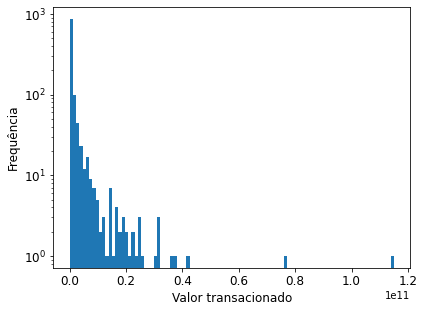
\includegraphics[scale=0.7]{images/base-de-dados-23.1-valor-total-por-cnae.png}
    \label{fig:pandemia:base-de-dados-23.1-valor-total-por-cnae}
    \fdadospesquisa
\end{figure}

Os dados de valores transacionados por CNAE tem grande variância, o que dificulta uma análise, mas é possível ver através do histograma que novamente os meses de abril e maio possuem uma distribuição de valores ligeiramente menor que o restante, mantendo o padrão anterior.

\begin{figure}[htb]
	\centering
    \caption{Diagrama de caixa dos valores mensais transacionados por CNAE no período analisado}
    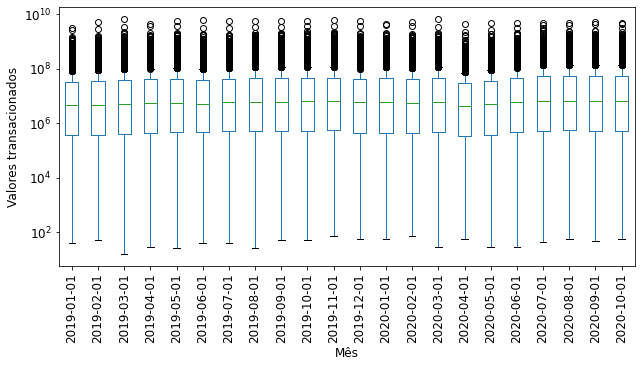
\includegraphics[scale=0.7]{images/base-de-dados-23.2-valor-mensal-por-cnae.png}
    \label{fig:pandemia:base-de-dados-23.2-valor-mensal-por-cnae}
    \fdadospesquisa
\end{figure}

Sobre os dados de CNAE também foi aplicada uma regressão linear sobre os dados obtidos nos meses de janeiro de 2019 a fevereiro de 2020 para a previsão dos valores para os meses de março de a outubro de 2020. Da mesma forma, a Tabela~\ref{tab:pandemia:impacto-por-cnae} mostra uma categorização de impacto mensal e total para CNAEs usando os mesmos critérios apresentados anteriormente: é considerado impacto mensal aquele onde para um determinado mês o valor obtido é 25\% menor que o valor previsto, e impacto total se o valor total obtido é menor que o previsto.

\begin{table}[htb]
\centering
\caption{Quantidade de CNAEs impactadas negativamente pela pandemia em relação às variações mensais ou totais}
\label{tab:pandemia:impacto-por-cnae}
    \begin{tabular}{l|r|r}
        \toprule
        Impacto & Mensal & Total \\
        \midrule
        Sim & 852 & 600 \\
        Não & 273 & 525 \\
        \bottomrule
    \end{tabular}
\fdadospesquisa
\end{table}

\section{Conclusões}
\label{section:impacto:conclusoes}

Finalizamos então a análise de impacto para diferentes segmentações, e pudemos verificar que em todos os cenários houve algum impacto entre os valores previstos e obtidos. Foi apresentada uma análise comparativa entre 2019 e 2020, e uma análise usando uma previsão de valor transacionado e valor real obtido. O impacto foi mais localizado entre os meses de março e junho, tornando o segundo trimestre de 2020 o mais afetado.

Cada cenário possui proporções diferentes de entidades afetadas e não afetadas pela pandemia, com um desbalanceamento maior para entidades afetadas. O objetivo, portanto, foi apresentar uma categorização das entidades ao mesmo tempo que aprofundamos a análise do Capítulo~\ref{chapter:base-de-dados} para mostrar sob o ponto de vista de valores transacionados uma nova perspectiva dos dados aqui apresentados.
